%Om Ganesayanamaha
\section{Apriori Algorithm for Declare Discovery}\label{sec:Apriori}

Standard techniques for the discovery of Declare constraints generate a set of candidate constraints by instantiating Declare templates with all the combinations of activities in the process. However, even for smaller processes, there can be millions of potential constraints.
Therefore, we adopt ideas from the well-known Apriori algorithm \cite{agrawalApriori}
for discovering combinations of activities frequently occurring in the same process execution.

Let $\Sigma$ be the set of potential activities. Let $\textbf{t} \in \Sigma^*$ be a trace over $\Sigma$, i.e., a sequence of activities executed for some process instance.
An event log $\mathcal{L}$ is a multi-set over $\Sigma^*$, i.e., a trace can appear multiple times in an event log.

The {\em support} of a set of activities is a measure that assesses the relevance of this set in an event log.
\begin{definition}[Support of an activity set]
The support of an activity set $A \subseteq \Sigma$ in an event log $\mathcal{L} = [\textbf{t}_1, \textbf{t}_2, \dots,  \textbf{t}_n]$
is the fraction of process instances in $\mathcal{L}$ that contain all of the activities in $A$, i.e.,\\
\begin{equation*}
\mathit{supp}(A) = \frac{\vert\mathcal{L}_{A}\vert}{\vert \mathcal{L}\vert}, \text{ where }\mathcal{L}_{A} = [\textbf{t} \in \mathcal{L} \mid \forall_{\texttt{x} \in A} \ \texttt{x} \in \textbf{t}]
\end{equation*}
\end{definition}
An activity set is considered to be {\em frequent} if its support is above a given threshold $\mathit{supp}_{\min}$. Let $\mathcal{A}_k$ denote the set of all frequent activity sets of size $k \in \mathbb{N}$ and let $\mathcal{C}_k$ denote the set of all {\em candidate activity sets} of size $k$ that may potentially be frequent. The Apriori algorithm uncovers all frequent activity sets in an event log. The algorithm starts by considering activity sets of size $1$ and progresses iteratively by considering activity sets of increasing sizes in each iteration and is based on the property {\em that any subset of a frequent activity set must be frequent}. The set of candidate activity sets of size $k+1$, $\mathcal{C}_{k+1}$, is generated by joining relevant frequent activity sets from $\mathcal{A}_k$. This set can be pruned efficiently using the property that a relevant candidate activity set of size $k+1$ cannot have an infrequent subset.
The activity sets in $\mathcal{C}_{k+1}$ that have a support above a given threshold $\mathit{supp}_{\min}$
constitute the frequent activity sets of size $k+1$ ($\mathcal{A}_{k+1}$) used in the next iteration.

 We explain the Apriori algorithm with an example. Consider an event log $\mathcal{L} =
 [
 \langle e, a, b, a, a, c, e \rangle,
 \langle e, a, a, b, c, e \rangle,
 \langle e, a, a, d, d, e \rangle,
 \langle b, b, c, c \rangle,
 \langle e, a, a, c, d, e \rangle]$
 defined over the set of activities $\Sigma = \{ a, b, c, d, e\}$.
 Let us try to find frequent activity sets whose support is above $50\%$.
 The Apriori algorithm starts by first considering activity sets of size $1$,
 i.e., the individual activities. The candidate sets in $\mathcal{C}_1$ correspond to the singletons of the elements of $\Sigma$.
 \figurename~\ref{fig:Apriorialgorithmexample}(a) depicts the candidate activity sets and their support.
 Among the candidate sets, activity $d$ has a support of only $40\%$ in the event log,
 which is below the specified threshold. Therefore, the frequent activity sets correspond to the singletons of the elements of
 $\Sigma\setminus\{ d \}$. In the next iteration, the Apriori algorithm considers
 candidate activity sets of size $2$, $\mathcal{C}_2$. Since the support of $d$ is less than the specified threshold,
 all activity sets that involve $d$ are bound to have their support less than the threshold.
 The Apriori algorithm elegantly captures this by deriving candidates at iteration $k+1$, $\mathcal{C}_{k+1}$,
 from frequent activity sets of iteration $k$. \figurename~\ref{fig:Apriorialgorithmexample}(b) depicts
 such candidate activity sets of size $2$ along with their support values. Only $4$ activity sets among
 $\mathcal{C}_2$ satisfy the minimum support criteria and hence are considered frequent
 (see $\mathcal{A}_2$ in \figurename~\ref{fig:Apriorialgorithmexample}(b)).
 Proceeding further, we get only one frequent activity set of size $3$ as
 depicted in \figurename~\ref{fig:Apriorialgorithmexample}(c). The algorithm
 terminates after this step as no further candidates can be generated.
 The frequent activity sets in $\mathcal{L}$ are $\mathcal{A}_1 \cup \mathcal{A}_2 \cup \mathcal{A}_3$.
 \begin{figure}[!t]
 \centering
 %\subfigure[Activity Set Size=1]{\includegraphics[width=0.23\textwidth]{Figures/AprioriIteration1}}
 %\subfigure[Activity Set Size=2]{\includegraphics[width=0.38\textwidth]{Figures/AprioriIteration2}}
 %\subfigure[Activity Set Size=3]{\includegraphics[width=0.38\textwidth]{Figures/AprioriIteration3}}
 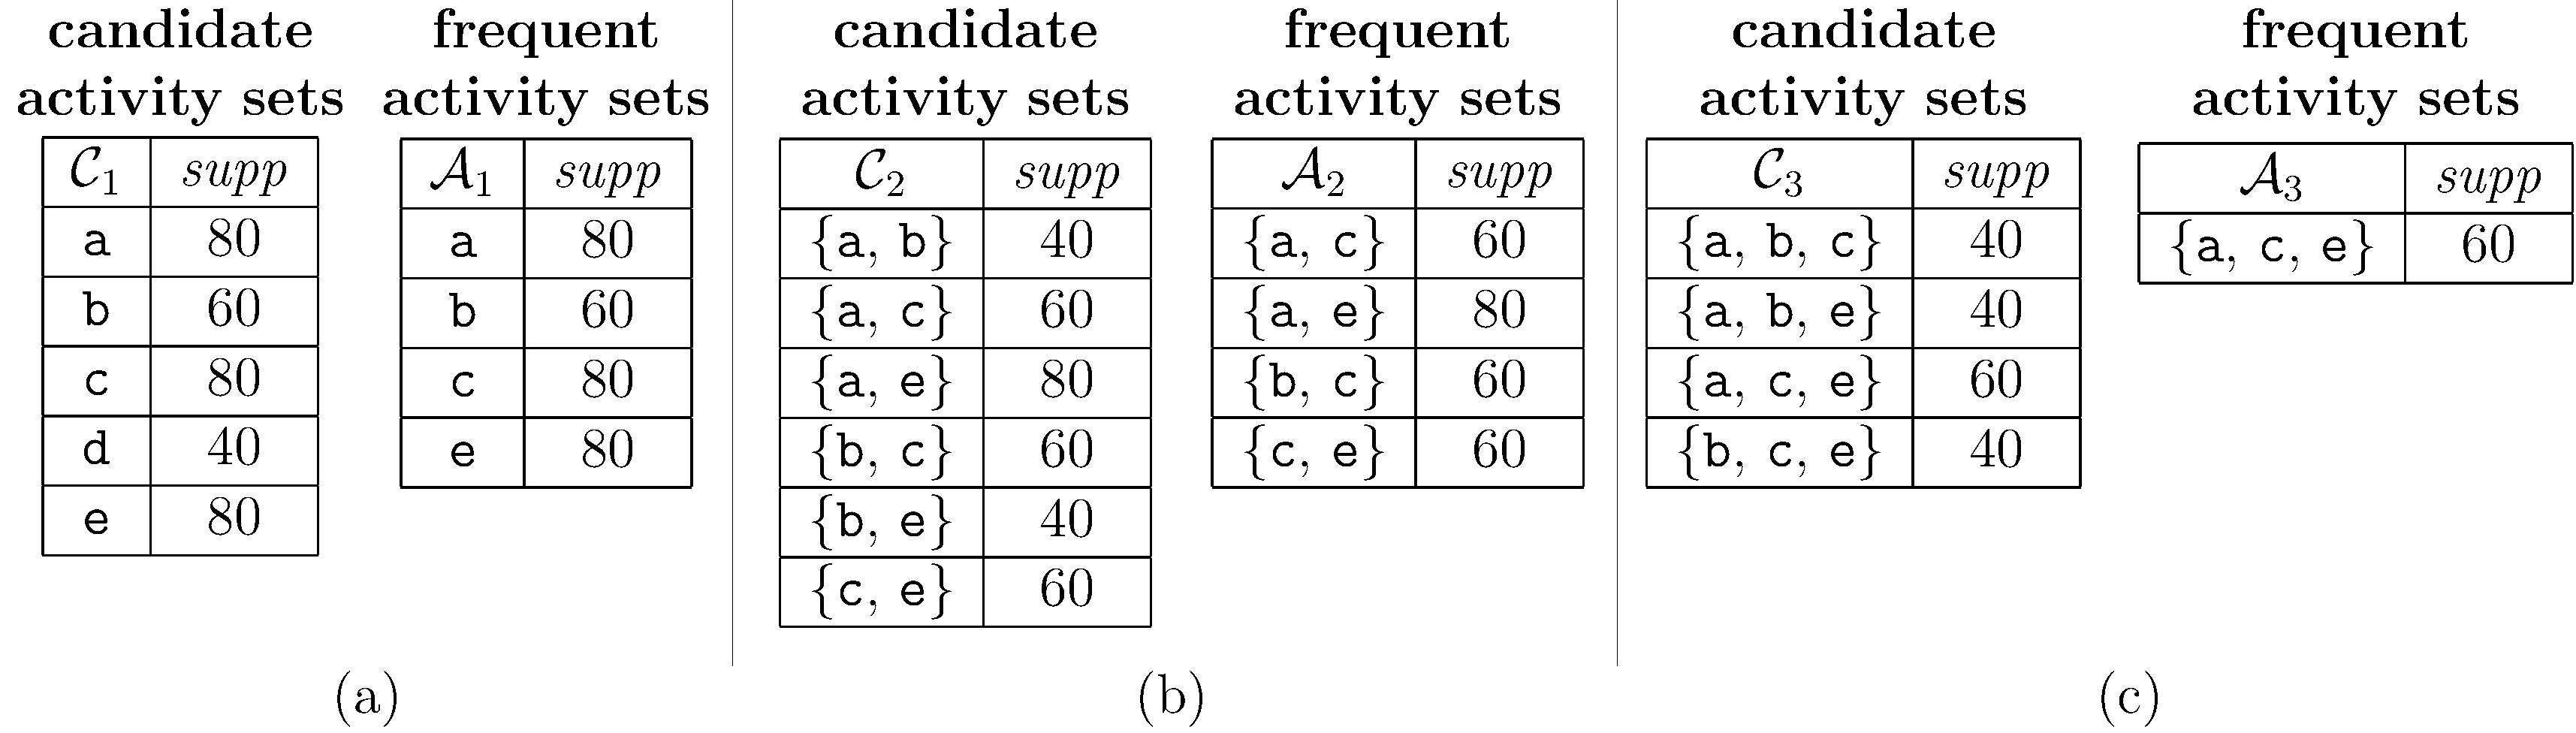
\includegraphics[width=0.99\textwidth]{images/AprioriExample}
 \caption{Discovering frequent activity sets using the Apriori algorithm in the event log $\mathcal{L}$. The support values are expressed in $\%$}
 \label{fig:Apriorialgorithmexample}
 \end{figure}

The Apriori algorithm returns frequent activity sets, which indicate that the activities involved
in an activity set are correlated. However, it doesn't specify the type of correlation.
Declare templates capture different relationships between activities. For instance,
for any frequent activity set $\{ a, b \}$, one can generate constraints such as the response $\square (a \rightarrow \lozenge b)$.


In general, to discover constraints deriving from a Declare template with $k$ parameters,
we have to generate frequent activity sets of size $k$. Afterwards, we generate the list of
candidate constraints. To do that, we instantiate the considered template by specifying
as parameters all the possible permutations of each frequent set. For instance, for the
frequent activity set $\{ a, b \}$, we generate the response constraints
$\square (a \rightarrow \lozenge b)$ and $\square (b \rightarrow \lozenge a)$.

Candidate constraints are checked with respect to the event log and only constraint with high constraint support are kept in the output Declare model. The {\em support} of a constraint is the ratio of traces in the event log in which the constraint holds.
\begin{definition}[Support of a constraint]
The support of a constraint $C$ in an event log $\mathcal{L} = [\textbf{t}_1, \textbf{t}_2, \dots,  \textbf{t}_n]$
is the fraction of traces in $\mathcal{L}$ in which $C$ holds, i.e.,\\
\begin{equation*}
\mathit{supp}(C) = \frac{\vert\mathcal{L}_{C}\vert}{\vert \mathcal{L}\vert}, \text{ where }\mathcal{L}_{C} = [\textbf{t} \in \mathcal{L} \mid C ~holds~in~t]
\end{equation*}
\end{definition}
 

%\marginpar{Here the original problem still exist. As discussed one could look a negative events (non-occurence). I assume this is left out for space reasons.}
%Limiting ourselves to frequent activity sets drastically reduces the number of candidate constraints to be checked.
%For instance, if we take the example in \figurename~\ref{fig:Apriorialgorithmexample}(b),
%to generate the candidate constraints deriving from a template with 2 parameters
%we consider all the permutations of each frequent activity set in $\mathcal{A}_2$ and we generate 12 candidate constraint (we also include pairs $(a, a)$, $(b, b)$, $(c, c)$, $(e, e)$ by considering repetitions of elements of frequent activity sets of size 1). In contrast, with the naive approach
%we need to consider all the dispositions of length 2 of 5 activities ($a, b, c, d, e$), i.e., 25 ($5^{2}$) candidate constraints.
%In general, to discover constraints deriving from a Declare template with $k$ parameters
%from a log with $n$ activities, the state space exploration using the naive approach
%always leads to $n^{k}$ candidate constraints. In contrast, applying our Apriori algorithm
%and considering only the frequent activity sets, the number of candidate constraints
%depends on the support value we specify for the Apriori algorithm. This number is
%often significantly lower than $n^{k}$ because we ignore the item sets with low support.
%


%{
%\begin{figure}[!b]
%\centering
%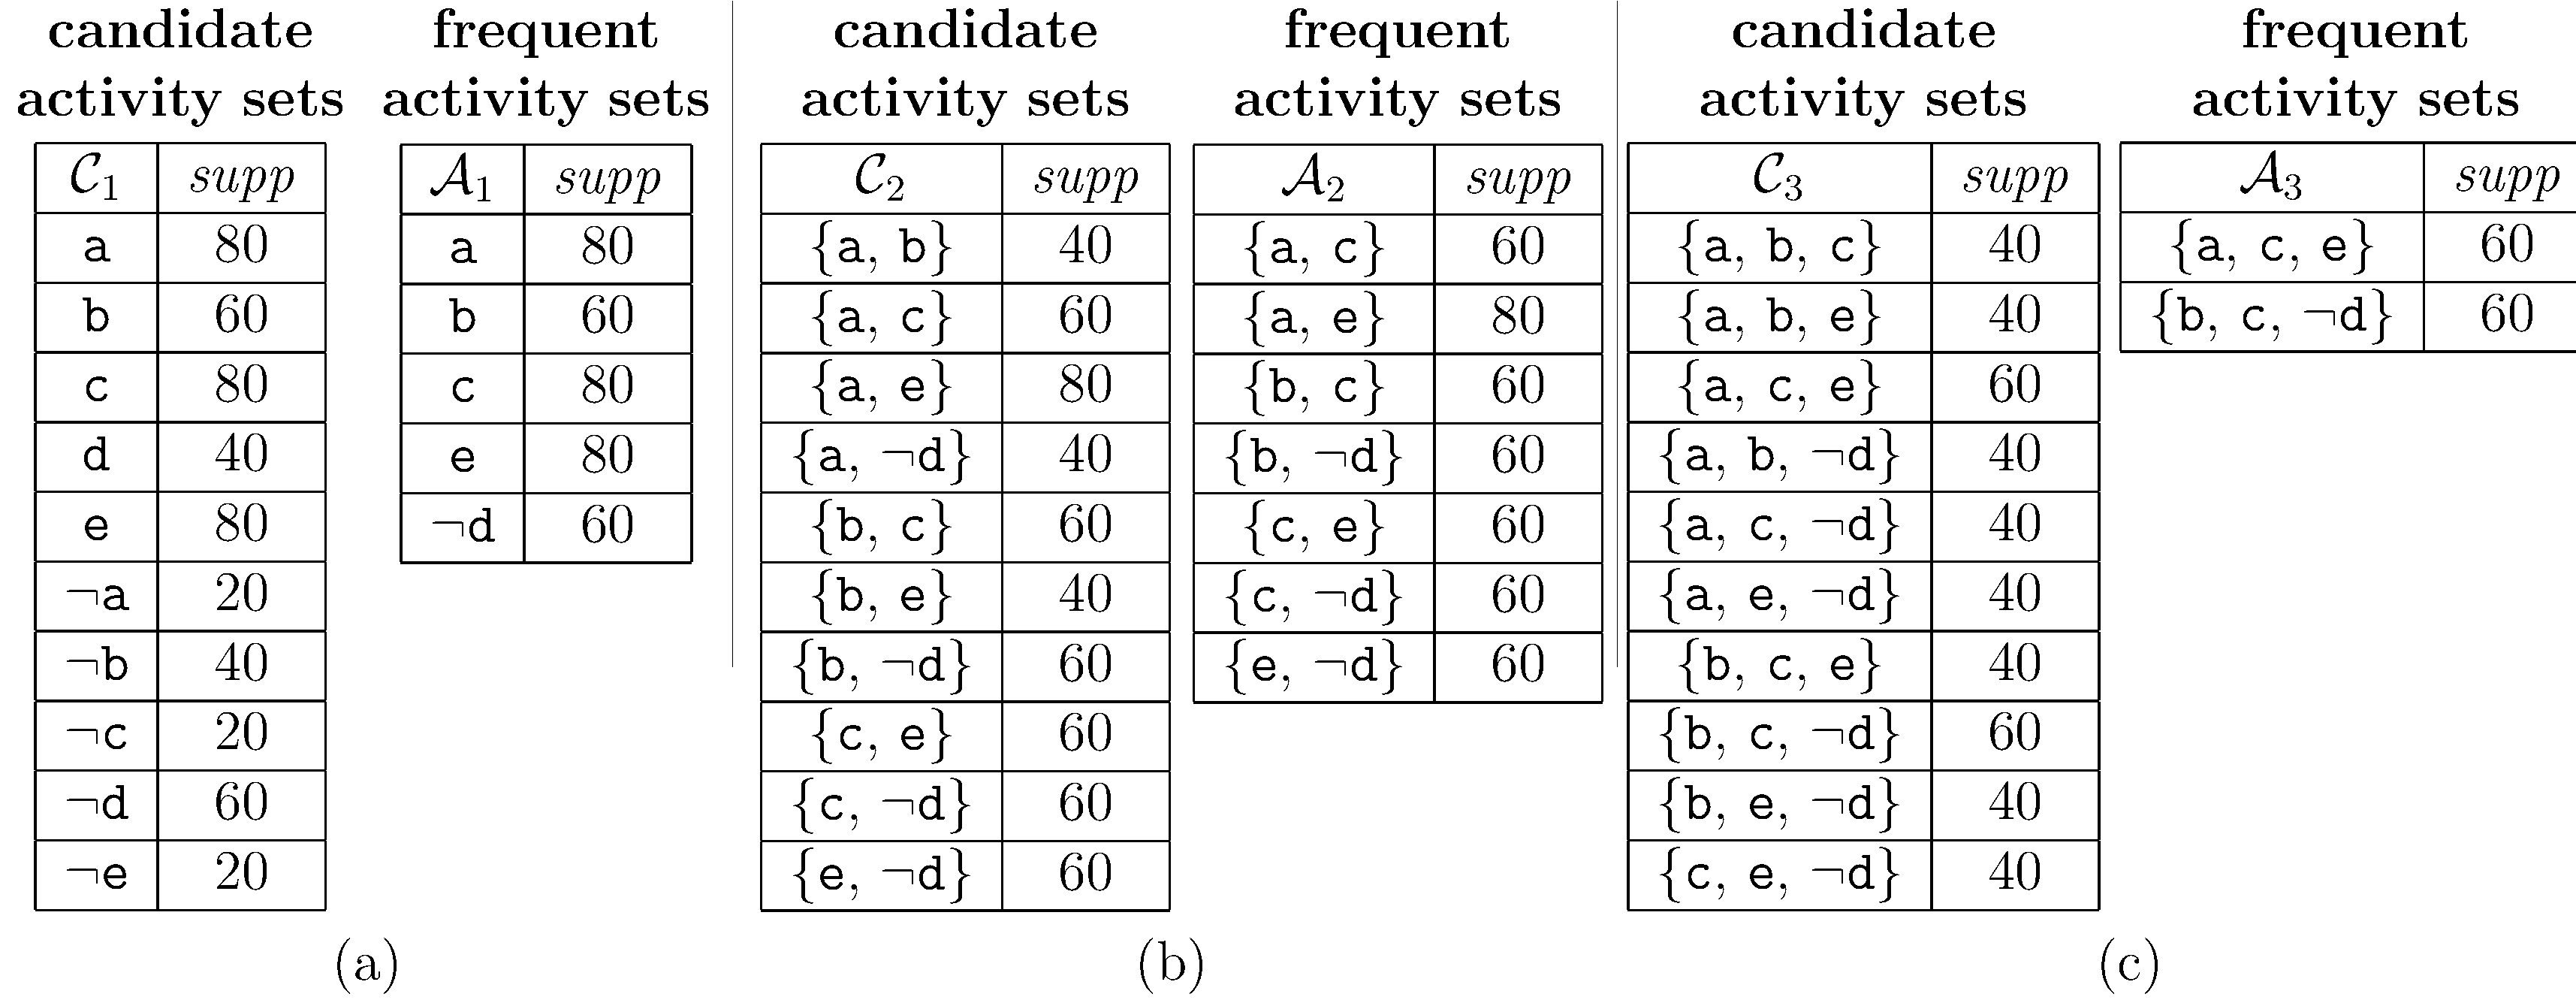
\includegraphics[width=0.99\textwidth]{images/AprioriExampleNegativeEvents}
%\caption{Discovering frequent activity sets considering negative (non-occurrence) events using the Apriori algorithm in the event log %$\mathcal{L}$. The support values are expressed in $\%$}
%\label{fig:ApriorialgorithmNegativeEventsExample}
%\end{figure}
%\vspace{-0.8cm}
%}
%\begin{table}[t!]
%\caption{Association rule formulation for some Declare constraints}
%\centering \scalebox{0.875}{
%\begin{tabular}{c|c|c|c|c}
%\textbf{\textit{template}}  & \textbf{\textit{LTL semantics}} & \textbf{\textit{rule}}  & \textbf{\textit{antecedent}} & %\textbf{\textit{consequent}}\\ \hline
%responded existence & $\lozenge a \rightarrow \lozenge b$ & {If $a$ occurs then $b$ occurs} &  {$a$} &  {$b$}\\ \hline
%\multirow{2}{*}{co-existence} & \multirow{2}{*}{$\lozenge a \leftrightarrow \lozenge b$} & If $a$ occurs then $b$ occurs $\wedge$ & %\multirow{2}{*}{$(a \vee b)$} & \multirow{2}{*}{$(a \vee b)$} \\
% & & If $b$ occurs then $a$ occurs~~~ & & \\ \hline
%response & $\square(a \rightarrow \lozenge b) $ & {If $a$ occurs then $b$ follows}  & {$a$} & {$b$}\\\hline
%$\square(a \rightarrow \lozenge b) $ & & & \\ \hline
%precedence & $(\neg b \sqcup a) \vee \square(\neg b)$ & {If $b$ occurs then $a$ precedes} &{$b$} & {$a$}\\\hline
%$(\neg b \sqcup a) \vee \square(\neg b)$ & & & \\\hline
%not succession & $\square(a \rightarrow \neg (\lozenge b))$ & {If $a$ occurs then $b$ does not follow}& {$a$}& {$b$} \\ \hline
%$\square(a \rightarrow \neg (\lozenge b))$ & & & \\ \hline
%\end{tabular}
%}
%\label{tab:rule}
%\vspace{-0.35cm}
%\end{table}
%One could also look at negative events (non-occurrence) within the Apriori setup. Such information might be useful for inferring, for instance, events that act as mutually exclusive, e.g., if $a$ occurs then $b$ does not occur.
%To facilitate this, we can also consider the negative events $\neg a$,
%for all $a \in \Sigma$. \figurename~\ref{fig:ApriorialgorithmNegativeEventsExample} depicts the discovery of frequent items sets
%considering non-occurrence of events using the apriori algorithm on the event log $\mathcal{L}$.
%Note that we now have additional frequent activity sets such as $\{b, c, \neg d\}$ signifying that if $b$ and $c$
%occurs then $d$ does not occur.

%
%This is reasonable because a Declare constraint between $a$ and $b$ is only activated
%in the process instances where both $a$ and $b$ occur \cite{Schunselaar2011}.\footnote{Throughout this paper the Declare templates taken into consideration are
%responded existence%($\lozenge a \rightarrow \lozenge b$)
%, co-existence%($\lozenge a \Leftrightarrow \lozenge b$)
%, response%($\square(a \rightarrow \lozenge b)$)
%, precedence%($(\neg b$ $U a)$ $\vee$ $\square(\neg b)$)
%, succession%(response(a, b) $\wedge$ precedence(a, b))
%, alternate response%($ \square ( a \rightarrow \bigcirc(\neg a$ $U b))$)
%, alternate precedence%(precedence(a, b) $\wedge \square ( b \rightarrow \bigcirc($precedence(a, b)$)) $)
%, alternate succession%(alternate response(a, b) $\wedge$ alternate precedence(a, b))
%, chain response%($\square(a \rightarrow \bigcirc b)$)
%, chain precedence%($\square(\bigcirc b \rightarrow a)$)
%, chain succession%($\square(a \Leftrightarrow \bigcirc b)$)
%, and not succession%($\square(a \rightarrow \neg (\lozenge b))$)
%. For constraints derived from all these templates the interesting
%witnesses are the process instances where the constraint holds
%and the vacuity detection condition ($\lozenge a \wedge \lozenge b$) is valid.}
%Therefore, since the item sets with low support rarely occur in the log, they are, for all constraints, less relevant.
%\marginpar{DISCUSS: This part is very questionable! First of all, I would be surprised if the vacuity detection conditions are indeed always $\lozenge a \wedge \lozenge b$.
%If so, why bother talking about it with so many words and references!
%Second, all of this does not hold for negative constraints.
%Two activities that exclude each other will not be found in this manner.}



